\section{Limited-memory quasi-Newton method}
Over this section we will explore one of the most popular and efficient algorithm of the quasi-Newton methods, we will show its convergence, complexity and, finally, we will analyze its performances on the LLS task.

\subsection{Overview on quasi-Newton methods}
The main feature of quasi-Newton methods, as opposed to pure Newton methods, is the fact that they do not need to compute the Hessian at each iteration and, therefore, are a cheaper solution, albeit coming with worse convergence speed.
\vspace{3mm}

\noindent First of all, let us introduce the following quadratic model of the objective function at the \textit{k-th} iteration, defined as
\begin{equation}
    m_k (p) = f_k + \nabla f_k^T p + \frac{1}{2} p^T B_k p
    \label{eq:bfgs_start}
\end{equation}
As we can see from \eqref{eq:bfgs_start}, we use $B_k$ as an approximation of the true Hessian matrix, which is typical in the context of the quasi-Newton methods. $B_k$ is an $n\times n$ symmetric positive definite matrix that is updated at each iteration.
\vspace{3mm}

\noindent We can explicitly write the minimizer $p_k$ (which indicates the search direction) of this convex quadratic model as
\begin{equation}
    p_k = -B_{k}^{-1} \nabla f_k
    \label{eq:bfgs_search_direction}
\end{equation}
The new step $k+1$ is defined as the following
\begin{equation}
    x_{k+1} = x_k + \alpha_k p_k
    \label{eq:bfgs_step}
\end{equation}
where $\alpha_k$ is the step length that should be chosen in order to satisfy the Wolfe conditions
\begin{subequations}
    \begin{equation}
        \label{eq:wolfe_c1}
        f(x_{k}+ \alpha p_{k}) \leq f(x_{k}) + c_1 \alpha_{k}p_{k}^{T}\nabla f(x_k),
    \end{equation}
    \begin{equation}
        \label{eq:wolfe_c2}
        -p_{k}^{T} \nabla f(x_{k} + \alpha_{k}p_{k}) \leq -c_2 p_{k}^{T}\nabla f(x_{k})
    \end{equation}
    with $0 < c_1 < c_2 < 1$.
\label{eq:wolfe_conditions}
\end{subequations}
\vspace{3mm}

\noindent Since our function is quadratic and convex, $\alpha_k$ can be actually computed by an exact line search in the following way
\begin{equation}
    \alpha_k = -\frac{\nabla f_k^T p_k}{p_k^TAp_k}
    \label{eq:lbfgs_alpha_exact}
\end{equation}
where $A=\hat{X}^T\hat{X}$, \eqref{eq:lbfgs_alpha_exact} was taken from chapter 3.5 by Nocedal et al. \cite{nocedal1999numerical}.
\vspace{3mm}

\noindent At the new iterate $x_{k+1}$, the model defined in \eqref{eq:bfgs_start} has gradient
\begin{equation}
    \nabla m_{k+1} (p) = \nabla f_{k+1} + p^T B_{k+1}
    \label{eq:bfgs_next_step_grad}
\end{equation}

\noindent The gradient of $m_{k+1}$ should match the one of the objective function $f$ at the latest two iterates $x_k$ and $x_{k+1}$. The second of these conditions is verified because $\nabla m_{k+1}(0) = \nabla f_{k+1}$, while the first one can be written as $\nabla m_{k+1}(-\alpha_k p_k)=\nabla f_k$, as defined in \eqref{eq:bfgs_next_step_grad}. By rearranging the latter we obtain 
\begin{equation}
    B_{k+1}\alpha_k p_k = \nabla f_{k+1} - \nabla f_k
    \label{eq:rearrange_grad}
\end{equation}
Now, lets define the displacement and the difference between gradients
\begin{equation}
    s_k = x_{k+1} - x_{k} = \alpha_k p_k, \hspace{3mm} y_k = \nabla f_{k+1} - \nabla f_k
    \label{eq:bfgs_displacement_gradient}
\end{equation}
then \eqref{eq:rearrange_grad} becomes
\begin{equation}
    B_{k+1}s_k = y_k
    \label{eq:bfgs_secant}
\end{equation}
The \eqref{eq:bfgs_secant} is known as the \textit{secant equation} and its purpose is to map $s_k$ into $y_k$, this is achievable iff the \textit{curvature condition} holds
\begin{equation}
    s_{k}^{T}y_k > 0
    \label{eq:bfgs_curvature}
\end{equation}
luckily for us, \eqref{eq:bfgs_curvature} always holds for convex functions like our case, so we can be sure that $B_{k+1}$ will inherit the positive definiteness from $B_k$.
\vspace{3mm}

\noindent To determine $B_{k+1}$ uniquely, an additional condition must be imposed such that among all symmetric matrices satisfying the secant equation we take the closest to the current matrix $B_k$. Knowing that $B=B^T$ and $By_k=s_k$, the condition is the following \footnotemark
\begin{equation}
    \displaystyle  \min_B \lVert B - B_k \rVert_W
    \label{eq:bfgs_closest_solution}
\end{equation}
\footnotetext{supposing that $\lVert A \rVert_W=\lVert W^{\frac{1}{2}}AW^{\frac{1}{2}} \rVert_F$ is the weighted Frobenius norm, where $W$ is any matrix such that $Ws_k=y_k$.}

\noindent We will discuss more deeply about one of the the quasi-Newton methods in section \ref{subsec:lbfgs}, where we will also show how to implement it.

\subsection{Limited memory BFGS}\label{subsec:lbfgs}
The chosen quasi-Newton algorithm is the BFGS method, named after its developers Broyden, Fletcher, Goldfarb, and Shanno, specifically we are going to implement a lighter in memory version of this called L-BFGS \cite{liu1989limited} which does not need save the entire Hessian approximation, but it updates the matrix by exploiting the previous $l$ iterations.
\vspace{3mm}

\noindent By introducing $H_k=B_k^{-1}$, we can impose the same conditions that $B_k$ had on $H_k$, therefore the latter must be symmetric and positive definite and should satisfy both \eqref{eq:bfgs_secant}, $H_ks_k=y_k$, and
\eqref{eq:bfgs_closest_solution}, hence
\begin{equation}
    \displaystyle  \min_H \lVert H - H_k \rVert_W
    \label{eq:bfgs_closest_solution_H}
\end{equation}
The $k+1$ step in \eqref{eq:bfgs_step}, now becomes
\begin{equation}
    x_{k+1} = x_k - \alpha_k H_k \nabla f_k
    \label{eq:bfgs_step_H}
\end{equation}
With a BFGS approach, H is then updated at every iteration by means of the following formula
\begin{equation}
    H_{k+1}=V_k^TH_kV_k+\rho_ks_ks_k^T
    \label{eq:bfgs_update_H}
\end{equation}
where
\begin{equation}
   \rho=\frac{1}{y_k^Ts_k}, \hspace{3mm} V_k=I-\rho_{k}s_{k}y_{k}^{T}
\end{equation}
\noindent Most of the times $H_k$ will be dense, hence the cost of storing and manipulating will be prohibitive when the number of variables becomes larger. The solution consists in dealing with a modified version of $H_k$ that stores $l$ vector pairs {$s_i$, $y_i$}.
\vspace{3mm}

\noindent The product $H_k \nabla f_k$ can be approximated by performing a sequence of products and vector summations involving the pairs $\{s_i, y_i\}$. After the new iterate is computed, the oldest vector pair in the set of pairs $\{s_i, y_i\}$ is replaced by the new pair $\{s_k , y_k\}$ obtained from \eqref{eq:bfgs_displacement_gradient}.
\vspace{3mm}

\noindent After choosing some initial Hessian approximation $H^{0}_{k}$ (that is allowed to vary from iteration to iteration) and by repeating \eqref{eq:bfgs_update_H}, we find that the $H_k$ satisfies the following

\begin{equation}
    \begin{aligned}
        H_k =& (V_{k-1}^{T} \dots V_{k-l}^{T}) H_{k}^{0}(V_{k-l} \dots V_{k-1}) \\
        &+ \rho_{k-l}(V_{k-1}^T \dots V_{k-l+1}^T) s_{k-l} s_{k-l}^T (V_{k-l+1} \dots V_{k+1}) \\
        &+ \rho_{k-l+1}(V_{k-1}^T \dots V_{k-l+2}^T) s_{k-l} s_{k-l+1}^T (V_{k-l+2} \dots V_{k+1}) \\
        &+ \dots \\
        &+ \rho{k-1}s_{k-1}s^{T}_{k-1}.
    \end{aligned}
    \label{eq:lbfgs_update_H}
\end{equation}
Thanks to (\ref{eq:lbfgs_update_H}) we can compute $H_k \nabla f_k$ in \eqref{eq:bfgs_step_H} with algorithm \ref{algorithm:lbfgs_compute_gradient}

\begin{algorithm}[H]
    \caption{L-BFGS two-loop recursion}
    \label{algorithm:lbfgs_compute_gradient}
    $q=\nabla f_k;$ \\
    \For{$i=k-1, k-2, \dots, k-l$}{
        $\alpha_i = \rho_i s_i^Tq;$ \\
        $q=q-\alpha_i y_i;$
    }
    $r=H_k^0q;$ \\
    \For{$i=k-l, k-l+1, \dots k-1$}{
        $\beta=\rho_i y_i^Tr;$ \\
        $r=r+s_i(\alpha_i-\beta);$
    }
    \textbf{return} $r;$
\end{algorithm}

\noindent A renowned method for choosing $H_{k}^{0}$ that has been proved effective in practice is to set $H_{k}^{0} = \gamma_k I$. $\gamma_k$ is the scaling factor that attempts to estimate the size of the true Hessian matrix along the most recent search direction and it is defined as
\begin{equation}
    \gamma_k = \frac{s_{k-1}^T y_{k-1}}{y_{k-1}^T y_{k-1}}
    \label{eq:lbfgs_initial_H}
\end{equation}

\noindent Algorithm \ref{algorithm:lbfgs_compute_gradient} has the advantage that the multiplication by the initial matrix $H_0^k$ is isolated from the rest of the computations, allowing this matrix to be chosen freely and to vary between iterations.

\begin{algorithm}[H]
    \caption{L-BFGS}
    \label{algorithm:lbfgs}
    Choose starting point $x_0$, integer $l > 0;$ \\
    $k = 0;$ \\
    \While{convergence not reached}{
        Choose $H_0;$ \\
        Compute $p_k = -H_k \nabla f_k$ from \autoref{algorithm:lbfgs_compute_gradient}; \\
        Compute $x_{k+1} = x_k + \alpha_k p_k$, where $\alpha_k$ is chosen by an exact line search; \\
        \If{$k > l$}{
            Discard the vector pair \{$s_{k-l}, y_{k-l}$\} from storage;
        }
        Compute and save $s_k \gets x_{k+1} - x_{k} , y_k = \nabla f_{k+1} - \nabla f_k ;$ \\
        $k = k+1;$
    }
\end{algorithm}

\subsection{Convergence and complexity}
It is already well-known that BFGS converges for convex minimization problems like LLS (we showed this property in \ref{subsec:introduction_convexity}), moreover, it has been shown that even L-BFGS converges on such tasks \cite{liu1989limited}, so we will not dive to much in details about all the literature about the convergence properties of such methods, but it is somewhat interesting showing the convergence rate of L-BFGS.
\vspace{3mm}

\noindent Keeping in mind that BFGS, and therefore its limited-memory verison, converges on strongly convex tasks, like LLS, since it satisfies the assumptions that \cite{nocedal1999numerical} states in theorem 6.5:
\begin{enumerate}
    \item \textit{The objective function f is twice continuously differentiable}, which is trivial as we know that $\nabla^2f=2\hat{X}^T\hat{X}$ and this is also positive definite.
    \item \textit{$B_k$ needs to be positive definite at each iteration}, this holds only if the \textit{curvature condition} defined by \eqref{eq:bfgs_curvature} is satisfied at each iteration, but, as we already stated, the latter always holds for convex functions so even this assumption is trivially fine for our case.
\end{enumerate}

\noindent From \cite{nocedal1999numerical} (section 6.4, until theorem 6.5) we can retrieve the fact that the convergence of the iterates is linear. In particular, the sequence $\lVert x_k - x^* \rVert$ converges to zero rapidly enough that
\begin{equation}
    \sum_{k=1}^{\infty} \lVert x_k - x^* \rVert < \infty
    \label{eq:lbfgs_conv_rate}
\end{equation}
where $x^*$ is the minimizer of the function.
\vspace{3mm}

\noindent First, we know that quasi-newton methods converge with superlinear rate under the existence of step length $\alpha_k$ that satisfies the Wolfe conditions \eqref{eq:wolfe_conditions}. The following theorem \ref{theorem:lbfgs_1} states the existence of such $\alpha_k$ (\cite{nocedal1999numerical}, theorem 3.6):
\begin{theorem}
    Suppose that $f : \mathbb{R}^{n} \xrightarrow{} \mathbb{R}$ is twice continuously differentiable. Consider the iteration $x_{k+1} = x_{k} + \alpha_k p_{k}$, where $p_k$ is a descent direction and $\alpha_k$ satisfies the Wolfe conditions with $c_1 \leq \frac{1}{2}$. If the sequence {$x_k$} converges to a point $x^*$ such that $\nabla f(x^*) = 0$ and $\nabla^2 f(x^*)$ is positive definite, and if the search direction satisfies
    \begin{equation}
        \lim_{k \xrightarrow{} \infty} \frac{\lVert \nabla f_k + \nabla^2 f_k p_k\rVert}{\lVert p_k \rVert} = 0,
        \label{eq:search_dir_limit}
    \end{equation}
    then \begin{enumerate}
        \item the step length $\alpha_k = 1$ is admissible for all $k$ greater than a certain index $k_0$; and
        \item if $\alpha_k = 1$ for all $k > k_0$, {$x_k$} converges to $x^*$ superlinearly.
    \end{enumerate}
    \label{theorem:lbfgs_1}
\end{theorem}

\noindent In quasi-Newton methods, applied in this case for LLS but this also works generally, since $p_k$ is the search direction of the form \eqref{eq:bfgs_search_direction} then \autoref{eq:search_dir_limit} can be rewritten as
\begin{equation}
    \lim_{k \xrightarrow{} \infty} \frac{\lVert (\mathbf{B}_k - \nabla^2 f(x^*))p_k\rVert}{\lVert p_k \rVert} = 0,
    \label{eq:lim_dir_quasi_newton}
\end{equation}

\noindent In order to obtain a superlinear convergence speed is enough that $\mathbf{B}_k$ become increasingly accurate approximations to $\nabla^2 f(x^*)$ along the search directions $p_k$. Importantly, condition \eqref{eq:lim_dir_quasi_newton} is \textit{both necessary and sufficient} for the superlinear convergence of quasi-Newton methods in convex cases thanks to \autoref{theorem:lbfgs_2} (\cite{nocedal1999numerical}, theorem 3.7).
\begin{theorem}
    Suppose that $f : \mathbb{R}^{n} \xrightarrow{} \mathbb{R}$ is twice continuously differentiable. Consider the iteration $x_{k+1} = x_k + p_k$ (that is, the step length $\alpha_k$ is uniformly 1) and that $p_k$ is given by \eqref{eq:bfgs_search_direction}. Let us assume also that {$x_k$} converges to a point $x^*$ such that $\nabla f(x^*) = 0$ and $\nabla^2 f(x^*)$ is positive definite. Then {$x_k$} converges superlinearly if and only if \eqref{eq:lim_dir_quasi_newton} holds.
    \label{theorem:lbfgs_2}
\end{theorem}

\noindent The main issue is that we can not safely assert \eqref{eq:lim_dir_quasi_newton} holds for our case, but making the assumption that the Hessian matrix $G(x)=\nabla^2f(x)$ is Lipschitz continuous at $x^*$, that is
\begin{equation}
    \lVert G(x)-G(x^*)\rVert \leq L\lVert x - x^*\rVert
    \label{eq:lbfgs_hessian_assumption}
\end{equation}
for every $x$ near $x^*$ where L is a positive constant, then \autoref{theorem:lbfgs_3} (from \cite{nocedal1999numerical}, theorem 6.6) comes in help for us.
\begin{theorem}
     Suppose that $f$ is twice continuously differentiable and that the iterates generated by the BFGS algorithm converge to a minimizer $x^*$ at which \eqref{eq:lbfgs_hessian_assumption} holds. Suppose also that \eqref{eq:lbfgs_conv_rate} holds. Then $x_k$ converges to $x^*$ at a superlinear rate.
     \label{theorem:lbfgs_3}
\end{theorem}

\noindent In our case, the first assumption is verified
\begin{equation}
    \lVert 2 \hat{X}^T \hat{X} - 2 \hat{X}^T \hat{X} \rVert = 0 \leq L \lVert x - x^* \rVert
\end{equation}
The second assumption holds as described in \cite{nocedal1999numerical}, section 6.4.
\vspace{3mm}

\noindent Both assumptions of \autoref{theorem:lbfgs_3} are satisfied, therefore we can state that L-BFGS converges superlinearly and, subsequently, thanks to \autoref{theorem:lbfgs_2}, \eqref{eq:lim_dir_quasi_newton} holds.

\paragraph{Complexity} The interesting part is the role that $l$ assumes on the convergence rate of the method. Keeping in mind that the memory/time cost per iteration is $\mathcal{O}(ln)$ \cite{nocedal1999numerical}, $l$ represents a trade-off in the convergence rate:
\begin{itemize}
    \item with small $l$, the convergence tends to be like the gradient approach.
    \item with large $l$, the convergence tends to be like the standard Newton methods.
\end{itemize}
During our analysis in \ref{subsec:lbfgs_analysis} we will show the aforementioned trade-off by using different values for $l$.

\subsection{Performance analysis} \label{subsec:lbfgs_analysis}
In this subsection we will show the results achieved by our implementation of the L-BFGS method by also showing empirically its superlinear convergence.
The hyper-parameters considered are the following:
\begin{itemize}
    \item $l \in \{5, 10, 15, 20\}$.
    \item $\lambda \in \{1e+4, 1e+2, 1, 1e-2, 1e-4\}$.
    \item the tolerance for $\lVert \nabla f \rVert$ was chosen to be $1e-14$.
    \item the maximum number of iterations was set to $1000$.
    \item the starting point was chosen to be $w_0=0$, since we have seen empirically to be the best choice when $\hat{X}$ becomes ill-conditioned.
\end{itemize}
For a total of $20$ configurations and each of one of them was run ten times in order to obtain the averages and the standard deviation, for a more reliable analysis.
\vspace{3mm}

\noindent The considered metrics are:
\begin{itemize}
    \item Relative error $\frac{\lVert w-w^*\rVert}{\lVert w^*\rVert}$, where $w^*$ is the solution obtained using the Matlab solver $\hat{X}\backslash\hat{y}$. $w$ can be used in this case instead of $f(w)$ thanks to fact that the global optimum $w^*$ is unique, see \ref{subsec:introduction_convexity} for a deeper understanding.
    \item Relative residual, $\frac{\lVert \hat{X}w-\hat{y} \rVert}{\lVert \hat{y} \rVert}$.
    \item Execution time.
    \item Number of iterations.
\end{itemize}
For correctness, we will first show in \autoref{tab:lbfgs_results} the results and then we will go deeper into to the other aspects by displaying the plots.
\begin{table}[H]
\centering
\begin{tabular}{c|c|c|c|c}
\hline \hline
l & $\lambda$ & Residual & Error & Iterations \\ \hline \hline

\rowcolor{gray!30} 5 & $10^4$ & $9.9 \times 10^{-1} \pm 5.74 \times 10^{-5}$ & $3.48 \times 10^{-14} \pm 2.15 \times 10^{-14}$ & 4 $\pm$ 0 \\ \hline

5 & $10^2$ & $8.68 \times 10^{-1} \pm 1.39 \times 10^{-2}$ & $2.82 \times 10^{-14} \pm 1.64 \times 10^{-14}$ & 10 $\pm$ 0 \\ \hline

\rowcolor{gray!30} 5 & 1 & $5.77 \times 10^{-2} \pm 5.80 \times 10^{-3}$ & $3.24 \times 10^{-12} \pm 8.77 \times 10^{-13}$ & 28 $\pm$ 14 \\ \hline

5 & $10^{-2}$ & $5.88 \times 10^{-4} \pm 6.02 \times 10^{-5}$ & $5.36 \times 10^{-12} \pm 2.32 \times 10^{-12}$ & 29 $\pm$ 10 \\ \hline

\rowcolor{gray!30} 5 & $10^{-4}$ & $5.80 \times 10^{-6} \pm 1.65 \times 10^{-7}$ & $6.30 \times 10^{-12} \pm 7.09 \times 10^{-13}$ & 26 $\pm$ 8 \\ \hline

10 & $10^4$ & $9.99 \times 10^{-1} \pm 3.02 \times 10^{-4}$ & $3.28 \times 10^{-14} \pm 2.69 \times 10^{-14}$ & 4 $\pm$ 0 \\ \hline

\rowcolor{gray!30} 10 & $10^2$ & $9.2 \times 10^{-1} \pm 9.37 \times 10^{-2}$ & $4.76 \times 10^{-15} \pm 7.90 \times 10^{-16}$ & 10 $\pm$ 0 \\ \hline

10 & 1 & $4.64 \times 10^{-2} \pm 2.34 \times 10^{-3}$ & $5.67 \times 10^{-14} \pm 7.72 \times 10^{-15}$ & 14 $\pm$ 0 \\ \hline

\rowcolor{gray!30} 10 & $10^{-2}$ & $5.11 \times 10^{-4} \pm 1.06 \times 10^{-4}$ & $4.80 \times 10^{-14} \pm 1.57 \times 10^{-14}$ & 14 $\pm$ 0 \\ \hline

10 & $10^{-4}$ & $5.85 \times 10^{-6} \pm 5.75 \times 10^{-7}$ & $3.18 \times 10^{-14} \pm 2.92 \times 10^{-15}$ & 14 $\pm$ 0 \\ \hline

\rowcolor{gray!30} 15 & $10^4$ & $9.99 \times 10^{-1} \pm 3.60 \times 10^{-4}$ & $3.27 \times 10^{-14} \pm 2.97 \times 10^{-14}$ & 4 $\pm$ 0 \\ \hline

15 & $10^2$ & $9.07 \times 10^{-1} \pm 6.69 \times 10^{-2}$ & $6.42 \times 10^{-14} \pm 4.89 \times 10^{-16}$ & 10 $\pm$ 0 \\ \hline

\rowcolor{gray!30} 15 & 1 & $5.12 \times 10^{-2} \pm 6.35 \times 10^{-3}$ & $2.41 \times 10^{-14} \pm 9.32 \times 10^{-15}$ & 13 $\pm$ 0 \\ \hline

15 & $10^{-2}$ & $4.96 \times 10^{-4} \pm 8.81 \times 10^{-5}$ & $4.28 \times 10^{-14} \pm 2.69 \times 10^{-14}$ & 13 $\pm$ 0 \\ \hline

\rowcolor{gray!30} 15 & $10^{-4}$ & $3.95 \times 10^{-6} \pm 2.17 \times 10^{-7}$ & $3.26 \times 10^{-14} \pm 7.74 \times 10^{-15}$ & 13 $\pm$ 0 \\ \hline

20 & $10^4$ & $9.99 \times 10^{-1} \pm 9.09 \times 10^{-4}$ & $1.40 \times 10^{-14} \pm 2.63 \times 10^{-15}$ & 4 $\pm$ 0 \\ \hline

\rowcolor{gray!30} 20 & $10^2$ & $9.37 \times 10^{-1} \pm 2.69 \times 10^{-2}$ & $5.62 \times 10^{-15} \pm 1.42 \times 10^{-15}$ & 10 $\pm$ 0 \\ \hline

20 & 1 & $5.89 \times 10^{-2} \pm 3.58 \times 10^{-3}$ & $1.73 \times 10^{-14} \pm 8.87 \times 10^{-16}$ & 13 $\pm$ 0 \\ \hline

\rowcolor{gray!30} 20 & $10^{-2}$ & $5.02 \times 10^{-4} \pm 1.82 \times 10^{-5}$ & $2.72 \times 10^{-14} \pm 3.60 \times 10^{-15}$ & 13 $\pm$ 0 \\ \hline

20 & $10^{-4}$ & $6.08 \times 10^{-6} \pm 4.01 \times 10^{-7}$ & $4.07 \times 10^{-14} \pm 3.04 \times 10^{-14}$ & 13 $\pm$ 0 \\ \hline \hline
\end{tabular}
\caption{L-BFGS results}
\label{tab:lbfgs_results}
\end{table}

\noindent Analyzing the results in \autoref{tab:lbfgs_results} it is evident that increasing the memory $l$ will lower the number of iteration and will result in a smaller error, since having a bigger $l$ means that we are able to approximate the Hessian better and, therefore, have a better descent direction.
\vspace{3mm}

\noindent We will talk about the effects of $l$ and $\lambda$ in \ref{subsubsec:lbfgs_l_analysis} and \ref{subsubsec:lbfgs_lambda_analysis} where we will show the convergence plots with our results. Furthermore, we will not plot the relative residual, but by looking at \autoref{tab:lbfgs_results}, we can see that it decreases when the error increases, this is typical when working with ill-conditioned matrices.
\vspace{3mm}

\noindent Before we dive deeper into the analysis, we have to recall that we showed the super-linear convergence of L-BFGS theoretically, we now aim to show it empirically through our plots. First, we need to mention that the error achieved by our method step by step is plotted alongside the linear and quadratic convergence rates, the former and the latter are defined as the following
\begin{equation}
    linear_k = \{ initErr,\frac{initErr}{2}, \frac{initErr}{4},\frac{initErr}{8},\frac{initErr}{16},\dots,\frac{initErr}{2^k} \}
\end{equation}
for the linear convergence rate and
\begin{equation}
    quadratic_k = \{ initErr, \frac{initErr}{4}, \frac{initErr}{16},\frac{initErr}{256},\frac{initErr}{65536},\dots,\frac{initErr}{2^{2^k}} \}
\end{equation}
for the quadratic one, $initErr$ is the initial error for both cases.

\subsubsection{Analysis on \texorpdfstring{$l$}{{}}} \label{subsubsec:lbfgs_l_analysis}
As we know, the memory size $l$ assumes an important role on the convergence rate, since for low values of $l$ the method achieves an almost linear rate, while an high value emulates the behavior of the Newton methods. For showing this we opted to plot the results of our method considering a case in which $\lambda=1$ as we can see in \autoref{fig:lbfgs_l_comparison}.
\begin{figure}[H]
    \centering
    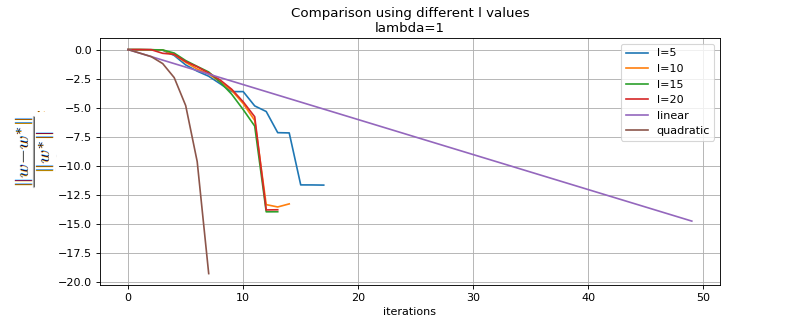
\includegraphics[width=0.8\linewidth]{images/lbfgs/lambda1.png}
    \caption{Convergence plot with $\lambda=1$ at different values of $l$}
    \label{fig:lbfgs_l_comparison}
\end{figure}

\noindent The chosen $l$ values were taken from the suggested ones by Nocedal \cite{nocedal1999numerical}, that is those inside the range $[3, 20]$ for keeping a good compromise between used memory and execution time, since we have already seen that $l$ influences the number of iterations and, therefore, the execution time of the method. We can also notice from \autoref{tab:lbfgs_results} that larger values of $l$ implies a smaller error (more evident when working with ill-conditioned matrices), this comes at no surprise since, as we already know, the more memory we use the more the Hessian is accurately approximated.
\vspace{3mm}

\noindent It's easy to notice from \autoref{fig:lbfgs_l_comparison} that for a smaller $l$ the convergence gets a little bit closer to the linear rate, meanwhile for bigger values it stays, more or less, in the middle, suggesting a super-linear convergence of the method. In our case the method was so fast that there were no relevant changes for $l>5$, since the algorithm does not reach enough iterations to show the real effect of such hyper-parameter.

\subsubsection{Analysis on \texorpdfstring{$\lambda$}{{}}} \label{subsubsec:lbfgs_lambda_analysis}
Analyzing the behavior at various values of $\lambda$ is extremely interesting and fundamental, as it explains what we will see over the plots in this subsection and in the rest of this report. The results can be briefly explained by the following observations
\begin{itemize}
    \item For larger values of $\lambda$ ($1e4$ and $1e2$) the method converges in few steps and obtains excellent results;
    \item For small $\lambda$, the algorithm requires more steps and the results get worse.
\end{itemize}

\noindent Such behavior arises when our matrix is ill-conditioned, that is when $\lambda$ is extremely small. This is caused by the fact that $\lambda$ is the smallest singular value  of $\hat{X}$ (see \ref{appendix:smallest_singular_value} and \ref{appendix:condition_number} for a better understanding) and, therefore, has a strong influence on the condition number of $\hat{X}$ making the method very unstable.

\begin{figure}[H]
    \centering
    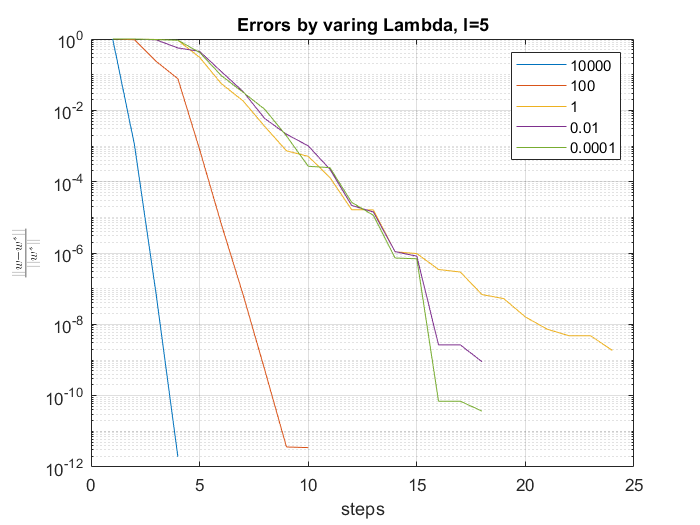
\includegraphics[width=0.8\linewidth]{images/lbfgs/errors_lambda.png}
    \caption{Errors by varying $\lambda$ with $l=5$.}
    \label{fig:lbfgs_errors_comparison_lambda}
\end{figure}

\noindent As we can see from \autoref{fig:lbfgs_errors_comparison_lambda}, the greater $\lambda$ is the better the algorithm converges even achieving a quadratic convergence rate (see \autoref{fig:lbfgs_1e4_l} for a better view) and maintaining a super-linear one for small values, confirming our previous observations and what we have stated for the convergence of L-BFGS. More plots of the L-BFGS method can be found in \ref{appendix:lbfgs_plots}.
